% !Mode:: "TeX:UTF-8"
% !TEX program  = xelatex

%\documentclass{cumcmthesis}
\documentclass[withoutpreface,bwprint]{cumcmthesis} %去掉封面与编号页

\usepackage{url}   % 网页链接
\usepackage{subcaption} % 子标题
\usepackage{cases}
\title{全国大学生数学建模竞赛编写的 \LaTeX{} 模板}
\tihao{A}
\baominghao{4321}
\schoolname{XX大学}
\membera{}
\memberb{向左}
\memberc{哈哈}
\supervisor{老师}
\yearinput{2017}
\monthinput{08}
\dayinput{22}

\title{二维椭圆型方程的差分格式 ~\\ ~\\ \normalsize 肖名财 \quad 刘礼海}
\begin{document}
	\maketitle
	\section{引言}
	各种物理性质的许多稳定过程都归结为椭圆形偏微分方程,诸如定常热传导问题和扩散问题、导体中电流分布问题、静电学和静磁学问题、弹性理论和渗流理论问题等等。
	
	椭圆型方程边值问题的精确解只在一些特殊情况下求得。有些问题即使求得他的解析解,但计算往往也很复杂,因此必须善于近似地求解这些问题。
	
	较具代表性得椭圆型方程是二维Poisson方程	
\begin{equation}
	-(\dfrac{\partial^2{u}}{\partial{x^2}}+\dfrac{\partial^2{u}}{\partial{y^2}})=f(x,y) ,\quad (x,y) \in \Omega \label{1}
\end{equation}
和Laplace方程
\begin{equation}
-(\dfrac{\partial^2{u}}{\partial{x^2}}+\dfrac{\partial^2{u}}{\partial{y^2}})=0 ,\quad (x,y) \in \Omega \label{2}
\end{equation}
其中$\Omega$为$R^2$中的一个有界区域。

定解条件通常有三类(Dirichlet边界条件、Neumann边界条件、第三类边值条件),我们主要考虑Dirichlet边值问题

\begin{subequations}
	\begin{numcases}{}
	-\Delta u=f(x,y),\quad  (x,y) \in \Omega \label{3a}\\
	u=\varphi(x,y),\quad (x,y) \in \tau \label{3b}
	\end{numcases}
\end{subequations}
其中$\Delta u=\dfrac{\partial^2{u}}{\partial{x^2}}+\dfrac{\partial^2{u}}{\partial{y^2}}$,为简单起见,考虑$\Omega$为矩形区域
\begin{equation}
\Omega = \{(x,y)|a \textless x \textless ,c \textless y \textless d\} \label{4}
\end{equation}

\section{数值格式}
将区间[a,b]作m等分,记$h_1=\dfrac{b-a}{m},x_i=a+ih_1,0 \leq i \leq m $

将区间[c,d]作n等分,记$h_2=\dfrac{d-c}{n},y_j=c+jh_2,0 \leq j \leq n $

分别称$h_1$为x方向的步长,$h_2$为y方向的步长,用两簇平行线
\begin{equation}
x=x_i,0 \leq i \leq m
\end{equation}
\begin{equation}
y=y_j,0 \leq j \leq n
\end{equation}

将区域$\Omega$剖分为mn个小矩形,称两簇直线的交点($x_i,y_j$)为网格节点。

我们称$i=0,i=m,j=0,j=n$处的节点为边界节点,记为$\gamma$,其余的节点为内节点,记为$\omega$。

\subsection{五点差分格式}
在节点$(x_i,y_j)$处考虑边值问题(\ref{3a}),(\ref{3b})有
\begin{subequations}
	\begin{numcases}{}
	-[\dfrac{\partial^2{u}}{\partial{x^2}}(x_i,y_j)+\dfrac{\partial^2{u}}{\partial{y^2}}(x_i,y_j)]=f(x_i,y_j) \quad (i,j) \in \omega \label{7a} \\
	u(x_i,y_j)=\varphi(x_i,y_j) \quad (i,j) \in \gamma \label{7b}
	\end{numcases}
\end{subequations}

用二阶中心差商代替二阶导数
\begin{equation}
\label{e1}
-\Delta hu_{i,j}=-[\dfrac{u_{i+1,j}-2u_{i,j}+u_{i-1,j}}{h_1^2}+\dfrac{u_{i,j+1}-2u_{i,j}+u_{i,j-1}}{h_2^2}]=f_{i,j}
\end{equation}

其中$u_{i,j}$为节点(i,j)上的网函数。导出截断误差,由Taylor展开
\begin{equation}
\label{e2}
\dfrac{u_{i+1,j}-2u_{i,j}+u_{i-1,j}}{h_1^2}=\dfrac{\partial{u(x_i,y_j)}}{\partial{x^2}}+\dfrac{h_1^2}{12}\dfrac{\partial^4{u(x_i,y_j)}}{\partial{x^4}}+\dfrac{h_1^4}{360}\dfrac{\partial^6{u(x_i,y_j)}}{\partial{x^6}}+O(h_1^6)
\end{equation}

\begin{equation}
\label{e3}
\dfrac{u_{i,j+1}-2u_{i,j}+u_{i,j-1}}{h_1^2}=\dfrac{\partial{u(x_i,y_j)}}{\partial{y^2}}+\dfrac{h_2^2}{12}\dfrac{\partial^4{u(x_i,y_j)}}{\partial{y^4}}+\dfrac{h_2^4}{360}\dfrac{\partial^6{u(x_i,y_j)}}{\partial{y^6}}+O(h_2^6)
\end{equation}

差分算子$-\Delta h$的截断误差
\begin{equation}
\label{e4}
R_{i,j}(u)=\Delta u(x_i,y_j)-\Delta hu(x_i,y_j)=-\dfrac{1}{12}[h_1^2\dfrac{\partial^4{u}}{\partial{x^4}}+h_2^2\dfrac{\partial^4{u}}{\partial{y^4}}]+O(h^4)=O(h^2)
\end{equation}

去掉截断误差,然后加上边值条件,得到如下差分格式
\begin{subequations}
	\begin{numcases}{}
	-[\dfrac{u_{i+1,j}-2u_{i,j}+u_{i-1,j}}{h_1^2}+\dfrac{u_{i,j+1}-2u_{i,j}+u_{i,j-1}}{h_2^2}]=f_{i,j} \quad (i,j) \in \omega \label{e5_a} \\
	u_{i,j}=\varphi(x_i,y_j) \quad (i,j) \in \gamma \label{e5_b}
	\end{numcases}
\end{subequations}

截断误差为$O(h^2)$.

称(\ref{e5_a})-(\ref{e5_b})为五点差分格式.

注:

(1)若$h_1=h_2=h_3$,则(\ref{e5_a})可简化为
\begin{equation}
\label{e6}
u_{i,j}-\dfrac{1}{4}(u_{i-1,j}+u_{i+1,j}+u{i,j-1}+u_{i,j+1})=\dfrac{h^2}{4}f_{i,j}
\end{equation}

(2)若$f \equiv 0$(Laplace方程),则(\ref{e5_a})可简化为
\begin{equation}
\label{e7}
u_{i,j}=\dfrac{1}{4}(u_{i-1,j}+u_{i+1,j}+u{i,j-1}+u_{i,j+1})
\end{equation}

我们将(\ref{e5_a})整理得
\begin{equation}
\label{e8}
-\dfrac{1}{h_2^2}u_{i,j-1}-\dfrac{1}{h_1^2}u_{i-1,j}+2(\dfrac{1}{h_1^2}+\dfrac{1}{h_2^2})u_{i,j}-\dfrac{1}{h_1^2}u_{i+1,j}-\dfrac{1}{h_2^2}u_{i,j+1}=f_{i,j}
\end{equation}

写成矩阵形式
\begin{equation}
\label{e9}
Au=f
\end{equation}

其中
$$
A=
\begin{bmatrix}
D & C \\
C & D & C \\
& \ddots & \ddots & \ddots \\
& & 	C & D
\end{bmatrix}
$$


$$
D=
\begin{bmatrix}
2(\dfrac{1}{h_1^2}+\dfrac{1}{h_2^2}) & -\dfrac{1}{h_2^2} \\
-\dfrac{1}{h_2^2} & 2(\dfrac{1}{h_1^2}+\dfrac{1}{h_2^2}) & -\dfrac{1}{h_2^2} \\
& \ddots & \ddots & \ddots \\
& & 	-\dfrac{1}{h_2^2} & 2(\dfrac{1}{h_1^2}+\dfrac{1}{h_2^2})
\end{bmatrix}
$$

$$
C=
\begin{bmatrix}
-\dfrac{1}{h_1^2} &  \\
 & -\dfrac{1}{h_1^2} & \\
&  & \ddots &  \\
& & 	 & -\dfrac{1}{h_1^2}
\end{bmatrix}
$$

$$
u=
\begin{bmatrix}
u_{1,1},u_{1,2},\cdots,u_{1,n-1}\\
u_{2,1},u_{2,2},\cdots,u_{2,n-1}\\
\vdots\\
u_{m-2,1},u_{m-2,2},\cdots,u_{m-2,n-1}\\
u_{m-1,1},u_{m-1,2},\cdots,u_{m-1,n-1}
\end{bmatrix}
$$

解方程(\ref{e9}),可以得到数值解。

\subsection{九点差分格式}
同样类似五点差分格式,我们用二阶中心差商代替二阶导数,由Taylor展开得到(\ref{e2})、(\ref{e3})两式。

九点格式是为了得到更高精度的截断误差,因此我们将(\ref{e4})式中的$h^2$项由$u$转化为已知函数$f$得
\begin{equation}
\label{e10}
\Delta u(x_i,y_j)=\Delta u(x_i,y_j)+\dfrac{1}{12}(h_1^2\dfrac{\partial^4{u(x_i,y_j)}}{\partial{x^4}}+h_2^2\dfrac{\partial^4{u(x_i,y_j)}}{\partial{y^4}})+O(h^4)
\end{equation}

含由$h^2$的部分经转化变为
\begin{equation}
\label{e11}
\dfrac{1}{12}(h_1^2\dfrac{\partial^2}{\partial{x^2}}+h_2^2\dfrac{\partial^2}{\partial{y^2}})(\dfrac{\partial^2{u(x_i,y_j)}}{\partial{x^2}}+\dfrac{\partial^2{u(x_i,y_j)}}{\partial{y^2}})-
\dfrac{h_1^2+h_2^2}{12}\dfrac{\partial^4{u(x_i,y_j)}}{\partial{x^2}\partial{y^2}}+O(h^4)
\end{equation}

为了方便计算

我们将$u_{xx}^{''}(x_i,y_{j+1})$、$u_{xx}^{''}(x_i,y_j)$、$u_{xx}^{''}(x_i,y_{j-1})$分别记为$a$、$b$、$c$

而
\begin{equation}
\label{e12}
\dfrac{\partial^4{u(x_i,y_j)}}{\partial{x^2}\partial{y^2}}=\dfrac{a-2b+c}{h_2^2}+O(h_2^2)
\end{equation}

使用二阶中心差商代替二阶导数,所以
\begin{subequations}
	\begin{numcases}{}
	a=\dfrac{u(x_{i+1},y_{j+1})-2u(x_i,y_{j+1})+u(x_{i-1},y_{j+1})}{h_1^2} \label{e13_a}\\
		b=\dfrac{u(x_{i+1},y_j)-2u(x_i,y_j)+u(x_{i-1},y_j)}{h_1^2} \label{e13_b}\\
		c=\dfrac{u(x_{i+1},y_{j-1})-2u(x_i,y_{j-1})+u(x_{i-1},y_{j-1})}{h_1^2} \label{e13_c}
	\end{numcases}
\end{subequations}

使用(\ref{e13_a})、(\ref{e13_b})、(\ref{e13_c})替换(\ref{e12})中的$a$、$b$、$c$,然后带入到(\ref{e11})得
\begin{equation}
	\begin{split}
\label{e14}
-f(x_i,y_j)+O(h^4)=&[\dfrac{u(x_{i_1},y_j)-2u(x_i,y_j)+u(x_{i+1},y_j)}{h_1^2}+\dfrac{u(x_i,y_{j-1})-2u(x_i,y_j)+u(x_i,y_{j+1})}{h_2^2}]\\
&+\dfrac{1}{12}[4u(x_i,y_j)-2(u(x_i,y_{j+1})+u(x_i,y_{j-1})+u(x_{i+1,y_j})+u(x_i,y_{j+1}))+\\
&u(x_{i+1},y_{j-1})+u(x_{i+1},y_{j-1})+u(x_{i+1},y_{j+1})+u(x_{i-1},y_{j+1})]\dfrac{h_1^2+h_2^2}{h_1^2h_2^2}+\\
&\dfrac{1}{12}[h_1^2\dfrac{\partial^2{f(x_i,y_j)}}{\partial{x^2}}+h_2^2\dfrac{\partial^2{f(x_i,y_j)}}{\partial{y^2}}]
	\end{split}
\end{equation}

略去误差项,加上边值条件,得Poisson方程九点差分格式
\begin{subequations}
	\begin{numcases}{}
-[\dfrac{u_{i-1,j}-2u_{i,j}+u_{i+1,j}}{h_1^2}+\dfrac{u_{i,j+1}-2u_{i,j}+u_{i,j-1}}{h_2^2}]	\dfrac{h_1^2+h_2^2}{h_1^2h_2^2}=f_{i,j}+G \label{e15_a}\\
G=\dfrac{1}{12}[h_1^2f_{xx}^{''}(x_i,y_j)+h_2^2f_{yy}^{''}(x_i,y_j)] \label{e15_b}\\
 1 \leq i \leq m-1,1\leq j \leq n-1 \label{e15_c}\\
u(x_i,y_j)=\varphi_{i,j} \quad i,j \in \gamma \label{e15_d}
	\end{numcases}
\end{subequations}

截断误差为$ O(h^4) $.

将九点差分格式进行整理
\begin{equation}
\begin{split}
\label{e16}
f_{i,j}+G=&-k_1u_{i-1,j-1}+(2k_1-k2)u_{i-1,j}-k_1u_{i-1,j+1}+(2k_1-k_3)u_{i,j-1}+\\
&(2k_2+2k_3-4k_1)u_{i,j}+(2k_1-k_3)u_{i,j+1}-k_1u_{i+1,j-1}+\\
&(2k_1-k_2)u_{i+1,j}-k_1u_{i+1,j+1}
\end{split}
\end{equation}

其中,$k_1=\dfrac{h_1^2+h_2^2}{12h_1^2h_2^2}$\quad,$k_2=\dfrac{1}{h_1^2}$\quad,$k_3=\dfrac{1}{h_2^2}$

将(\ref{e16})写成矩阵形式
\begin{equation}
\label{e17}
Au=f
\end{equation}

其中
$$
A=
\begin{bmatrix}
D & C \\
C & D & C \\
& \ddots & \ddots & \ddots \\
& & 	C & D
\end{bmatrix}
$$


$$
D=
\begin{bmatrix}
2k_2+2k_3-4k_1 & 2k_1-k_3 \\
2k_1-k_3 & 2k_2+2k_3-4k_1 & -k_1 \\
& \ddots & \ddots & \ddots \\
& & 	2k_1-k_3 & 2k_2+2k_3-4k_1
\end{bmatrix}
$$

$$
C=
\begin{bmatrix}
2k_1-k_2 & -k_1 \\
-k_1 & 2k_1-k_2 & -k_1 \\
& \ddots & \ddots & \ddots \\
& & 	-k_1 & 2k_1-k_2
\end{bmatrix}
$$

$$
u=
\begin{bmatrix}
u_{1,1},u_{1,2},\cdots,u_{1,n-1}\\
u_{2,1},u_{2,2},\cdots,u_{2,n-1}\\
\vdots\\
u_{m-2,1},u_{m-2,2},\cdots,u_{m-2,n-1}\\
u_{m-1,1},u_{m-1,2},\cdots,u_{m-1,n-1}
\end{bmatrix}
$$

f要根据边界条件具体确定

解(\ref{e17}),即可得数值解。

\section{数值例子}
数值例子为
\begin{equation}
\left\{
\begin{array}{lcl}
-(\dfrac{\partial^2{u}}{\partial{x^2}}+\dfrac{\partial^2{u}}{\partial{y^2}})=(\pi^2-1)e^xsin(\pi y) &,&0 \textless x \textless 2,0 \textless y \textless 1 \\

u(0,y)=sin(\pi y) \quad u(2,y)=e^2sin(\pi y)&, & 0 \leq y \leq 1 \\

u(x,0)=0,u(x,1)=0,&, &0 \leq x \leq 2
\end{array}
\right.
\end{equation}

该问题的精确解为$e^xsin(\pi y)$.

定义误差为$$ E_{\infty}(h_1,h_2)=\max \limits_{1 \leq i \leq N_1-1 \atop 1 \leq j \leq N_2-1 } |u(x_{i},y_{j})-u_{i,j})| $$
现在分别使用两种数值格式对该例子进行求解,解题程序运行于Matlab 2018a.
\subsection{五点差分格式}
当$h_1=\dfrac{1}{16}$\quad$h_2=\dfrac{1}{16}$时的数值解和精确解见图\ref{fig:f1}和\ref{fig:f2},从图像上看很接近。

\begin{figure}[htbp]
	\begin{minipage}[htbp]{0.5\linewidth}
		\centering
		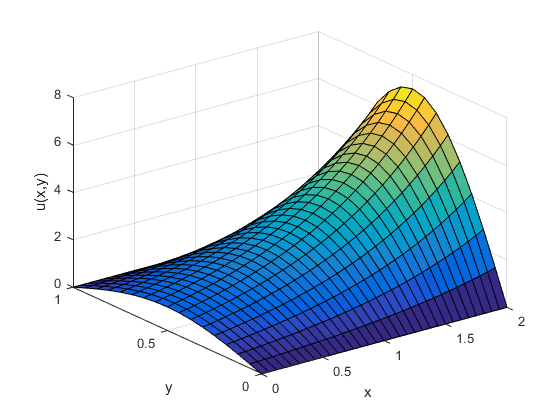
\includegraphics[width=1\linewidth]{figures/f1}
		\caption{$h_1=\dfrac{1}{16}$\quad$h_2=\dfrac{1}{16}$时的精确解}
		\label{fig:f1}
	\end{minipage}
	\begin{minipage}[htbp]{0.5\linewidth}
	\centering
	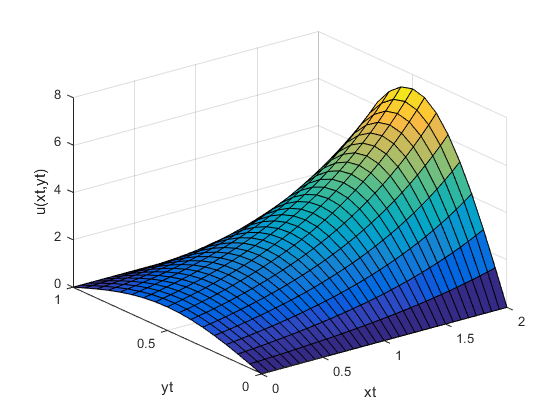
\includegraphics[width=1\linewidth]{figures/f2}
	\caption{$h_1=\dfrac{1}{16}$\quad$h_2=\dfrac{1}{16}$时的数值解}
	\label{fig:f2}
	\end{minipage}
\end{figure}


表1是不同步长下,部分节点的精确解和数值解的具体数值,我们看到随着步长的减小,数值解越接近精确解。
% Table generated by Excel2LaTeX from sheet 'Sheet1'
\begin{table}[htbp]
	\centering
	\caption{不同步长下部分节点的精确解与数值解}
	\begin{tabular}{cccccc}
			\toprule[1.5pt]
		($h_1$,$h_2$) & x=1/8,y=1/2 & x=3/8,y=1/2 & x=5/8,y=1/2 & x=7/8,y=1/2 & x=9/8,y=1/2 \\
		\midrule[1pt]
		1/8,1/8 & 1.1396038  & 1.4710228  & 1.8919087  & 2.4296181  & 3.1175586  \\
		1/16,1/16 & 1.1347613  & 1.4589884  & 1.8741409  & 2.4065360  & 3.0895320  \\
		1/32,1/32 & 1.1335502  & 1.4559860  & 1.8697125  & 2.4007821  & 3.0825377  \\
		1/64,1/64 & 1.1332460  & 1.4552319  & 1.8686005  & 2.3993379  & 3.0807831  \\
		精确解    & 1.1331480  & 1.4549919  & 1.8682465  & 2.3988759  & 3.0802171  \\
			\bottomrule[1.5pt]
	\end{tabular}%
	\label{tab:1}%
\end{table}%

取不同$h_1$ 和 $h_2$时的误差图\ref{fig:f3},图\ref{fig:f4},图\ref{fig:f5},图\ref{fig:f6},步长越小,误差也越小。
\begin{figure}[htbp]
	\begin{minipage}[htbp]{0.5\linewidth}
		\centering
		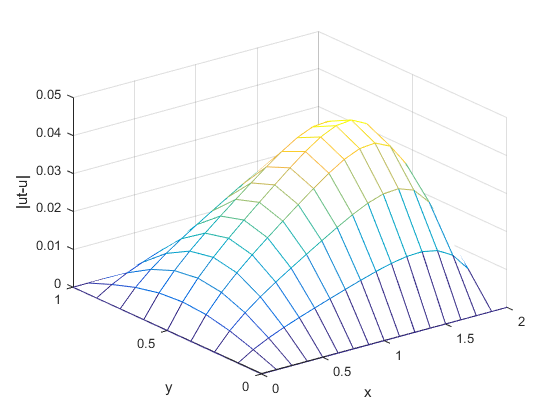
\includegraphics[width=1\linewidth]{figures/f3}
		\caption{$h_1=\dfrac{1}{8}$\quad$h_2=\dfrac{1}{8}$时的误差图}
		\label{fig:f3}
	\end{minipage}
	\begin{minipage}[htbp]{0.5\linewidth}
		\centering
		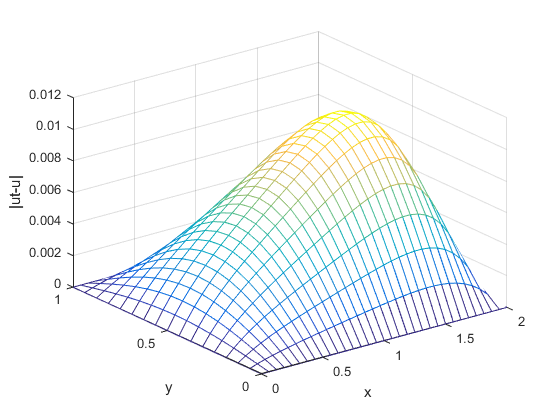
\includegraphics[width=1\linewidth]{figures/f4}
		\caption{$h_1=\dfrac{1}{16}$\quad$h_2=\dfrac{1}{16}$时的误差图}
		\label{fig:f4}
	\end{minipage}
	\begin{minipage}[htbp]{0.5\linewidth}
		\centering
		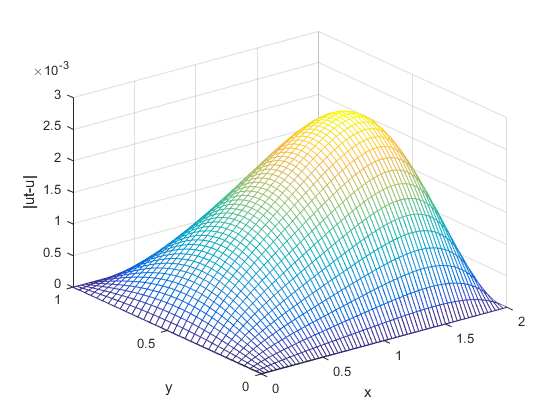
\includegraphics[width=1\linewidth]{figures/f5}
		\caption{$h_1=\dfrac{1}{32}$\quad$h_2=\dfrac{1}{32}$时的误差图}
		\label{fig:f5}
	\end{minipage}
	\begin{minipage}[htbp]{0.5\linewidth}
		\centering
		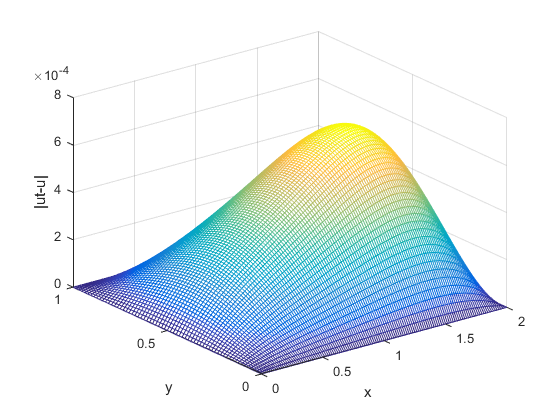
\includegraphics[width=1\linewidth]{figures/f6}
		\caption{$h_1=\dfrac{1}{64}$\quad$h_2=\dfrac{1}{64}$时的误差图}
		\label{fig:f6}
	\end{minipage}
\end{figure}
取不同步长时,最大误差和误差阶见表\ref{tab:2},误差阶为2阶,符合$O(h^2)$的截断误差

% Table generated by Excel2LaTeX from sheet 'Sheet1'
\begin{table}[htbp]
	\centering
	\caption{取不同步长是的最大误差和误差阶}
	\begin{tabular}{ccc}
			\toprule[1.5pt]
		($h_1$,$h_2$) & E($h_1$,$h_2$) & log(E($2h_1$,$2h_2$)) \\
			\midrule[1pt]
		1/8,1/8 & 4.2377E-02 & * \\
		1/16,1/16 & 1.0605E-02 & 1.99854  \\
		1/32,1/32 & 2.6505E-03 & 2.00042  \\
		1/64,1/64 & 6.5230E-04 & 2.02264  \\
		\bottomrule[1.5pt]
	\end{tabular}%
	\label{tab:2}%
\end{table}%


\subsection{九点差分格式}
当$h_1=\dfrac{1}{16}$\quad$h_2=\dfrac{1}{16}$时的数值解和精确解见图\ref{fig:f7}和\ref{fig:f8},从图像上看很接近。

\begin{figure}[htbp]
	\begin{minipage}[htbp]{0.5\linewidth}
		\centering
		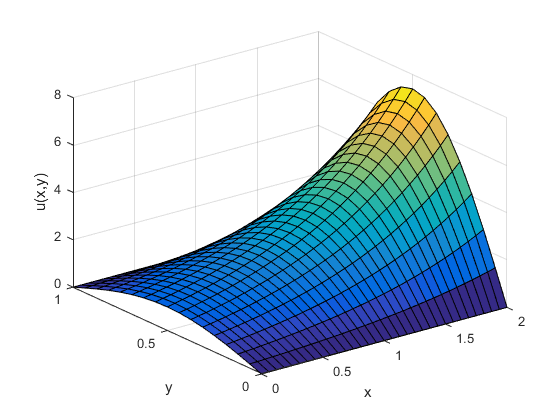
\includegraphics[width=1\linewidth]{figures/f7}
		\caption{$h_1=\dfrac{1}{16}$\quad$h_2=\dfrac{1}{16}$时的精确解}
		\label{fig:f7}
	\end{minipage}
	\begin{minipage}[htbp]{0.5\linewidth}
		\centering
		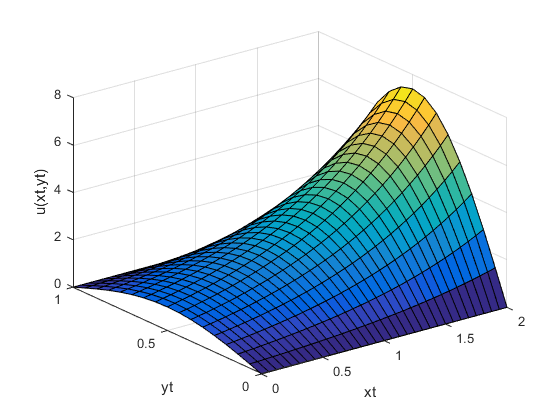
\includegraphics[width=1\linewidth]{figures/f8}
		\caption{$h_1=\dfrac{1}{16}$\quad$h_2=\dfrac{1}{16}$时的数值解}
		\label{fig:f8}
	\end{minipage}
\end{figure}


表\ref{tab:3}是不同步长下,部分节点的精确解和数值解的具体数值,我们看到随着步长的减小,数值解越接近精确解。
% Table generated by Excel2LaTeX from sheet 'Sheet1'
% Table generated by Excel2LaTeX from sheet 'Sheet1'
\begin{table}[htbp]
	\centering
	\caption{不同步长下部分节点的数值解与精确解($h_1=h_2$)}
	\begin{tabular}{cccccc}
		\toprule[1.5pt]
		($h_1$,$h_2$) & x=1/8,y=1/2 & x=3/8,y=1/2 & x=5/8,y=1/2 & x=7/8,y=1/2 & x=9/8,y=1/2 \\
		\midrule[1pt]
		1/8,1/8 & 1.1331304  & 1.4549467  & 1.8681801  & 2.3987897  & 3.0801127  \\
		1/16,1/16 & 1.1331473  & 1.4549886  & 1.8682419  & 2.3988700  & 3.0802104  \\
		1/32,1/32 & 1.1331484  & 1.4549912  & 1.8682457  & 2.3988750  & 3.0802164  \\
		1/64,1/64 & 1.1331484  & 1.4549914  & 1.8682459  & 2.3988753  & 3.0802168  \\
		精确解    & 1.1331485  & 1.4549914  & 1.8682460  & 2.3988753  & 3.0802168  \\
		\bottomrule[1.5pt]
	\end{tabular}%
	\label{tab:3}%
\end{table}%




取不同$h_1$ 和 $h_2$时的误差图\ref{fig:f9},图\ref{fig:f10},图\ref{fig:f11},图\ref{fig:f12},步长越小,误差也越小。因此通过增加点数(减小步长),可以增加值的精确性。
\begin{figure}[htbp]
	\begin{minipage}[htbp]{0.5\linewidth}
		\centering
		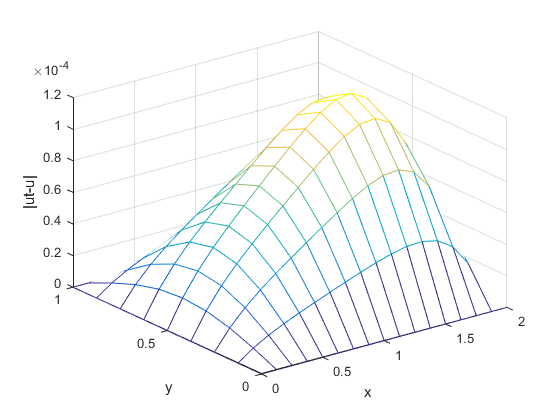
\includegraphics[width=1\linewidth]{figures/f9}
		\caption{$h_1=\dfrac{1}{8}$\quad$h_2=\dfrac{1}{8}$时的误差图}
		\label{fig:f9}
	\end{minipage}
	\begin{minipage}[htbp]{0.5\linewidth}
		\centering
		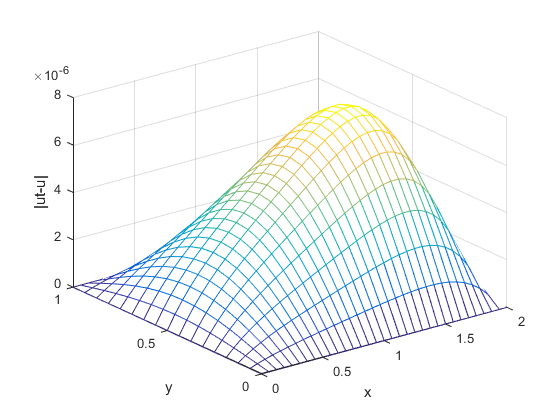
\includegraphics[width=1\linewidth]{figures/f10}
		\caption{$h_1=\dfrac{1}{16}$\quad$h_2=\dfrac{1}{16}$时的误差图}
		\label{fig:f10}
	\end{minipage}
	\begin{minipage}[htbp]{0.5\linewidth}
		\centering
		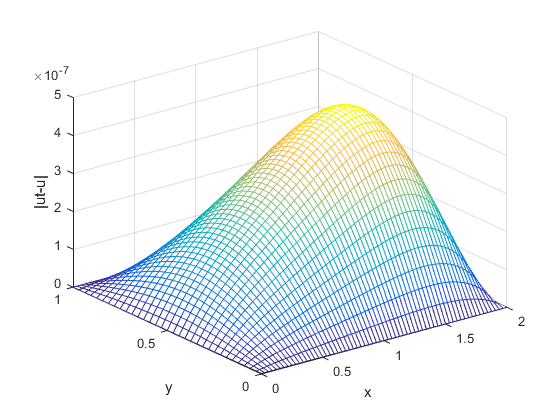
\includegraphics[width=1\linewidth]{figures/f11}
		\caption{$h_1=\dfrac{1}{32}$\quad$h_2=\dfrac{1}{32}$时的误差图}
		\label{fig:f11}
	\end{minipage}
	\begin{minipage}[htbp]{0.5\linewidth}
		\centering
		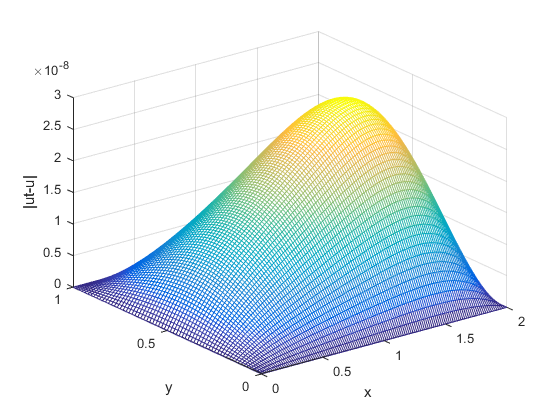
\includegraphics[width=1\linewidth]{figures/f12}
		\caption{$h_1=\dfrac{1}{64}$\quad$h_2=\dfrac{1}{64}$时的误差图}
		\label{fig:f12}
	\end{minipage}
\end{figure}

$h_1=h_2$时的最大误差和误差阶见表\ref{tab:4},误差阶为4阶,符合$O(h^4)$的截断误差

% Table generated by Excel2LaTeX from sheet 'Sheet1'
% Table generated by Excel2LaTeX from sheet 'Sheet1'
\begin{table}[htbp]
	\centering
	\caption{九点差分下的最大误差及误差阶($h_1=h_2$)}
	\begin{tabular}{ccc}
		\toprule[1.5pt]
		($h_1,h_2$) & E($h_1,h_2$) & log(E($2h_1,2h_2$)) \\
		\midrule[1pt]
		1/8,1/8 & 1.18580E-04 & * \\
		1/16,1/16 & 7.35587E-06 & 4.01082  \\
		1/32,1/32 & 4.59576E-07 & 4.00052  \\
		1/64,1/64 & 2.87191E-08 & 4.00022  \\
		\bottomrule[1.5pt]
	\end{tabular}%
	\label{tab:4}%
\end{table}%

同样我们还做了$h_1$>$h_2$和$h_1$<$h_2$时的最大误差和误差阶见表\ref{tab:5}和表\ref{tab:6}。
% Table generated by Excel2LaTeX from sheet 'Sheet1'
\begin{table}[htbp]
	\centering
	\caption{九点差分下的最大误差及误差阶($h_1$>$h_2$)}
	\begin{tabular}{ccc}
		\toprule[1.5pt]
		($h_1,h_2$) & E($h_1,h_2$) & log(E($2h_1,2h_2$)) \\
		\midrule[1pt]
		1/4,1/8 & 4.97132E-05 & * \\
		1/8,1/16 & 3.10557E-06 & 4.00070  \\
		1/16,1/32 & 1.94120E-07 & 3.99984  \\
		1/32,1/64 & 1.21572E-08 & 3.99706  \\
		\bottomrule[1.5pt]
	\end{tabular}%
	\label{tab:5}%
\end{table}%

% Table generated by Excel2LaTeX from sheet 'Sheet1'
\begin{table}[htbp]
	\centering
	\caption{九点差分下的最大误差及误差阶($h_1$<$h_2$)}
	\begin{tabular}{ccc}
		\toprule[1.5pt]
		($h_1,h_2$) & E($h_1,h_2$) & log(E($2h_1,2h_2$)) \\
		\midrule[1pt]
		1/8,1/4 & 2.49261E-03 & * \\
		1/16,1/8 & 1.50889E-04 & 4.04610  \\
		1/32,1/16 & 9.36919E-06 & 4.00942  \\
		1/64,1/32 & 5.84407E-07 & 4.00288  \\
		\bottomrule[1.5pt]
	\end{tabular}%
	\label{tab:6}%
\end{table}%

通过表\ref{tab:4},表\ref{tab:5},表\ref{tab:6}可知,误差阶接近4阶。并且随着步长的减小越精确。

\section{总结}
本文建立了两种二维椭圆型方程差分格式:五点差分格式和九点差分格式。用这两种格式,编写matlab程序,对具体的算例进行数值求解。五点差分格式的截断误差为  $ O(h^2) $,九点差分格式的截断误差为$O(h^4) $,精度为:九点差分格式 >五点差分格式。

%参考文献
\newpage
\begin{thebibliography}{9}%宽度9
	\bibitem[1]{1}
	李荣华. 偏微分方程数值解法[M]. 高等教育出版社, 2005.
	\bibitem[2]{2}
	孙志忠, 计算数学. 偏微分方程数值解法[M]. 科学出版社, 2005.
\end{thebibliography}

\newpage
%附录
\begin{appendices}
	\section{程序流程图}
	程序的流程见图\ref{fig:process}
	\begin{figure}[htbp]
		\centering
		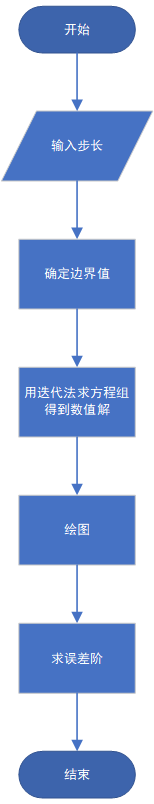
\includegraphics[width=0.2\linewidth]{figures/process}
		\caption{程序流程图}
		\label{fig:process}
	\end{figure}
	
	\section{五点差分格式代码}
	fu.m 求精确解
	\begin{lstlisting}[language=matlab]
	function  fh=fu(x,y)
	%精确解函数
	fh=exp(x).*sin(pi.*y);
	end
	\end{lstlisting}
	
	f.m 右端项
	\begin{lstlisting}[language=matlab]
	function ft= f(x,y)
	%右端函数
	ft=(pi^2-1)*exp(x)*sin(pi*y);
	end
	\end{lstlisting}
	
	ft.m 用五点差分格式求数值解
	\begin{lstlisting}[language=matlab]
	%五点差分格式,高斯赛德尔求解
	function  uf = ft(M,N)
	%步长
	h1=2/M;
	h2=1/N;
	%内节点
	x=h1:h1:2-h1;
	y=h2:h2:1-h2;
	uf=ones(M+1,N+1);
	u0=zeros(M+1,N+1);
	u1=zeros(M+1,N+1);
	%y边值
	y0=0:h2:1;
	u0(1,:)=sin(pi*y0);
	u0(M+1,:)=exp(2)*sin(pi*y0);
	%x边值
	u0(:,1)=0;
	u0(:,N+1)=0;
	u1=u0;
	while(1)
	for m=1:M-1
	for n=1:N-1
	u1(m+1,n+1)=(f(x(m),y(n))+u1(m+1,n)/h2^2+u1(m,n+1)/h1^2+...
	u0(m+2,n+1)/h1^2+u0(m+1,n+2)/h2^2)/(2*(1/h1^2+1/h2^2));
	end
	end
	if norm(u1-u0,'inf')<1e-6 
	uf=u1';break;
	else
	u0=u1;
	end
	end
	\end{lstlisting}
	
	wudianchafen.m 绘制误差图,精确解和数值解对比图以及误差和误差阶
	\begin{lstlisting}[language=matlab]
	clc;clear;
	%m,n为等分大小
	m=[16,32,64,128];
	n=[8,16,32,64];
	%步长1/8、1/16、1/32、1/64
	x1=0:2/m(1):2;x2=0:2/m(2):2;x3=0:2/m(3):2;x4=0:2/m(4):2;
	y1=0:1/n(1):1;y2=0:1/n(2):1;y3=0:1/n(3):1;y4=0:1/n(4):1;
	%精确解图像
	figure(1)
	%使用散点绘图,m=32,n=16的精确解图像
	[X,Y]=meshgrid(x2,y2);
	u=fu(X,Y);
	surf(X,Y,u);
	xlabel('x');ylabel('y');zlabel('u(x,y)');
	%m=32,n=16的数值解图像
	[Xt,Yt]=meshgrid(x2,y2);
	ut=ft(m(2),n(2));
	figure(2);
	surf(Xt,Yt,ut);
	xlabel('xt');ylabel('yt');zlabel('u(xt,yt)');
	%误差以及误差阶
	[X1,Y1]=meshgrid(x1,y1);
	[X2,Y2]=meshgrid(x2,y2);
	[X3,Y3]=meshgrid(x3,y3);
	[X4,Y4]=meshgrid(x4,y4);
	pt1=abs(fu(X1,Y1)-ft(m(1),n(1)));%误差
	pt2=abs(fu(X2,Y2)-ft(m(2),n(2)));
	pt3=abs(fu(X3,Y3)-ft(m(3),n(3)));
	pt4=abs(fu(X4,Y4)-ft(m(4),n(4)));
	%误差曲面图
	figure(3)
	mesh(X1,Y1,pt1);
	xlabel('x');ylabel('y');zlabel('|ut-u|');
	figure(4)
	mesh(X2,Y2,pt2);
	xlabel('x');ylabel('y');zlabel('|ut-u|');
	figure(5)
	mesh(X3,Y3,pt3);
	xlabel('x');ylabel('y');zlabel('|ut-u|');
	figure(6)
	mesh(X4,Y4,pt4);
	xlabel('x');ylabel('y');zlabel('|ut-u|');
	%最大误差
	maxpt1=max(pt1(:));
	maxpt2=max(pt2(:));
	maxpt3=max(pt3(:));
	maxpt4=max(pt4(:));
	%误差比例
	rate1=log2(maxpt1/maxpt2);
	rate2=log2(maxpt2/maxpt3);
	rate3=log2(maxpt3/maxpt4);
	%x取1/8、3/8、5/8、7/8、9/8和y取1/2处的精确解和数值解
	x0=[1/8,3/8,5/8,7/8,9/8];
	y0=1/2;
	%精确解
	f0=null(1);
	for i=1:5
	f0(i)=fu(x0(i),y0);
	end
	%数值解
	ut1=ft(m(1),n(1))';
	ut2=ft(m(2),n(2))';
	ut3=ft(m(3),n(3))';
	ut4=ft(m(4),n(4))';
	utf=ones(4,5);%记录部分节点的值
	for j=1:5
	utf(1,j)=ut1(m(1)/8*j,n(1)/2+1);
	utf(2,j)=ut2(m(2)/8*j-1,n(2)/2+1);
	utf(3,j)=ut3(m(3)/8*j-3,n(3)/2+1);
	utf(4,j)=ut4(m(4)/8*j-7,n(4)/2+1);
	end
	\end{lstlisting}
	
	\section{九点差分格式代码}
	fu.m 求精确解
	\begin{lstlisting}[language=matlab]
	function  fh=fu(x,y)
	%精确解函数
	fh=exp(x).*sin(pi.*y);
	end
	\end{lstlisting}
	
	f.m 右端项
	\begin{lstlisting}[language=matlab]
	function ft= f(x,y)
	%右端函数
	ft=(pi^2-1)*exp(x)*sin(pi*y);
	end
	\end{lstlisting}
	
	ft.m 用九点差分格式求数值解
	\begin{lstlisting}[language=matlab]
	%九点差分格式,高斯赛德尔求解
	function  uf = ft(M,N)
	%步长
	h1=2/M;
	h2=1/N;
	k1=(h1^2+h2^2)/(12*(h1^2)*(h2^2));
	k2=1/h1^2;
	k3=1/h2^2;
	%内节点
	x=h1:h1:2-h1;
	y=h2:h2:1-h2;
	uf=ones(M+1,N+1);
	u0=zeros(M+1,N+1);
	u1=zeros(M+1,N+1);
	%y边值
	y0=0:h2:1;
	u0(1,:)=sin(pi*y0);
	u0(M+1,:)=exp(2)*sin(pi*y0);
	%x边值
	u0(:,1)=0;
	u0(:,N+1)=0;
	u1=u0;
	while(1)
	for m=1:M-1
	for n=1:N-1
	u1(m+1,n+1)=(f(x(m),y(n))+1/12*(h1^2*f(x(m),y(n))+...
	h2^2*(pi^2-pi^4)*exp(x(m))*sin(pi*y(n)))+k1*...
	u1(m,n)-(2*k1-k2)*u1(m,n+1)+k1*u1(m,n+2)-...
	(2*k1-k3)*u1(m+1,n)-(2*k1-k3)*u0(m+1,n+2)+...
	k1*u0(m+2,n)-(2*k1-k2)*u0(m+2,n+1)+...
	k1*u0(m+2,n+2))/(2*k2+2*k3-4*k1);
	end
	end
	if norm(u1-u0,'inf')<1e-12
	uf=u1';break;
	else
	u0=u1;
	end
	end
	\end{lstlisting}
	
	jiudianchafen.m 绘制误差图,精确解和数值解对比图以及误差和误差阶
	\begin{lstlisting}[language=matlab]
	clc;clear;
	m=[16,32,64,128];
	n=[8,16,32,64];
	% m=[8,16,32,64];
	%n=[8,16,32,64];
	%m=[16,32,64,128];
	%n=[4,8,16,32];
	%步长1/8、1/16、1/32、1/64
	x1=0:2/m(1):2;x2=0:2/m(2):2;x3=0:2/m(3):2;x4=0:2/m(4):2;
	y1=0:1/n(1):1;y2=0:1/n(2):1;y3=0:1/n(3):1;y4=0:1/n(4):1;
	%精确解图像
	figure(1)
	%使用散点绘图,m=32,n=16的精确解图像
	[X,Y]=meshgrid(x2,y2);
	u=fu(X,Y);
	surf(X,Y,u);
	xlabel('x');ylabel('y');zlabel('u(x,y)');
	%m=32,n=16的数值解图像
	[Xt,Yt]=meshgrid(x2,y2);
	ut=ft(m(2),n(2));
	figure(2);
	surf(Xt,Yt,ut);
	xlabel('xt');ylabel('yt');zlabel('u(xt,yt)');
	%误差以及误差阶
	[X1,Y1]=meshgrid(x1,y1);
	[X2,Y2]=meshgrid(x2,y2);
	[X3,Y3]=meshgrid(x3,y3);
	[X4,Y4]=meshgrid(x4,y4);
	%的误差
	pt1=abs(fu(X1,Y1)-ft(m(1),n(1)));
	pt2=abs(fu(X2,Y2)-ft(m(2),n(2)));
	pt3=abs(fu(X3,Y3)-ft(m(3),n(3)));
	pt4=abs(fu(X4,Y4)-ft(m(4),n(4)));
	%误差曲面图
	figure(3)
	mesh(X1,Y1,pt1);
	xlabel('x');ylabel('y');zlabel('|ut-u|');
	figure(4)
	mesh(X2,Y2,pt2);
	xlabel('x');ylabel('y');zlabel('|ut-u|');
	figure(5)
	mesh(X3,Y3,pt3);
	xlabel('x');ylabel('y');zlabel('|ut-u|');
	figure(6)
	mesh(X4,Y4,pt4);
	xlabel('x');ylabel('y');zlabel('|ut-u|');
	%h1=h2最大误差
	maxpt1=max(pt1(:));
	maxpt2=max(pt2(:));
	maxpt3=max(pt3(:));
	maxpt4=max(pt4(:));
	%误差比例
	rate1=log2(maxpt1/maxpt2);
	rate2=log2(maxpt2/maxpt3);
	rate3=log2(maxpt3/maxpt4);
	%x取1/8、3/8、5/8、7/8、9/8和y取1/2处的精确解和数值解
	x0=[1/8,3/8,5/8,7/8,9/8];
	y0=1/2;
	%精确解
	f0=null(1);
	for i=1:5
	f0(i)=fu(x0(i),y0);
	end
	%数值解
	ut1=ft(m(1),n(1))';
	ut2=ft(m(2),n(2))';
	ut3=ft(m(3),n(3))';
	ut4=ft(m(4),n(4))';
	utf=ones(4,5);%记录部分节点的值
	for j=1:5
	utf(1,j)=ut1(m(1)/8*j,n(1)/2+1);
	utf(2,j)=ut2(m(2)/8*j-1,n(2)/2+1);
	utf(3,j)=ut3(m(3)/8*j-3,n(3)/2+1);
	utf(4,j)=ut4(m(4)/8*j-7,n(4)/2+1);
	end
	\end{lstlisting}
	
\end{appendices}

\end{document}